\paragraph{Notations}
\sequenceof{$A$} indicates a finite sequence, potentially empty, composed of
type $A$ elements. Sequences are thus defined as
\[
   \sequenceof{A} =
      \begin{cases}
         \lbrack \rbrack\\
         A :: \sequenceof{A}
      \end{cases}
\]
% REprendre notation avec pipe genre langage Elm, Caml.
The addition of an element $e$ at the head of a sequence $S$ is written
\pushfun{$e$}{$S$}, standing for $e:: S$. The retrieval and removal of the head
of a sequence $S$ is written \popfun{$S$}, returning $head(S)$ prior to applying
$S \gets tail(S)$. Lastly, \isemptyfun{$S$} indicates whether $S$ is
an empty sequence, and is equivalent to testing if $S = \lbrack \rbrack$.

\section{Components}%
\label{sec:cache_coherence_components}
\begin{figure}
\begin{center}
\begin{tabular}{cc}
\begin{subfigure}[t]{0.47\textwidth}
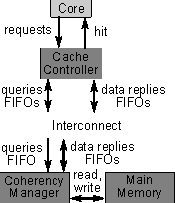
\includegraphics[width=14em]{\chapterdirectory/figure/cmp_overview.pdf}
\caption{Overview}%
\label{fig:cache-coherence-cmps-overview}
\end{subfigure} &
\begin{subfigure}[t]{0.47\textwidth}
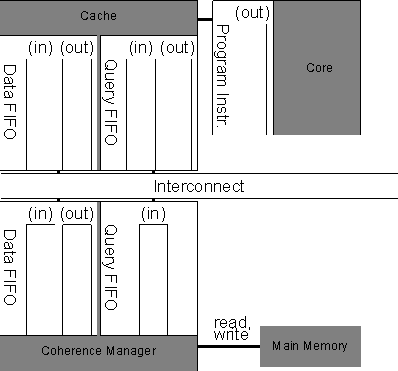
\includegraphics[width=20em]{\chapterdirectory/figure/cmp_detailed.pdf}
\caption{Showcasing the FIFOs}%
\label{fig:cache-coherence-cmps-fifos}
\end{subfigure}
\end{tabular}
\end{center}
\caption{Components involved in cache coherence}%
\label{fig:cache-coherence-cmps}
\end{figure}

In this section are presented the various components involved in maintaining
cache coherence in a multi-core architecture.
Figure~\ref{fig:cache-coherence-cmps} shows how the components presented in this
section are interconnected, with Figure~\ref{fig:cache-coherence-cmps-overview}
providing an overview and Figure~\ref{fig:cache-coherence-cmps-fifos} making
the involved FIFO queues more apparent.

Architectures generally feature instruction, data, as well as caches holding
both. Instruction caches are not affected by cache coherence and thus not
considered in this chapter.

\subsection{Memory Elements}%
\label{sec:memory_element}
The memory of a system is partitioned into addressable blocks. That is, there
are blocks of a certain size for which performing any access operation on its
content requires performing an operation on the block in its entirety.

Cache coherence is maintained over a cache line. Cache lines form another
partitioning of the system's main memory, such that all cache lines contain the
same amount of addressable blocks. Thus, even without accounting for the
possibility of multiple addresses pointing to the same atomic block, there may
be multiple addresses pointing to different parts of a same cache line. The
content of each cache line is made of contiguous memory blocks. Thus, if a
cache line of 16 elements starts with a block of address 42, it will also have
the blocks of addresses 43 through 57. If ignored, this mismatch between blocks
used for cache coherence and for program instructions can lead to unexpected
results, such as false sharing (see Appendix~\ref{app:false_sharing}).

To avoid unwarranted complications, this thesis merges the two partitioning
types into one: memory elements. In effect, we consider that memory elements
are cache lines with the size of a single addressable block, but change the
term so that this simplification remains explicit. Furthermore, since there is
only a single address per memory element, a memory element and its address can
be used interchangeably to refer to one another.

\begin{definition}[Memory Element]
\label{def:memoryelement}
The set of all memory elements is defined as $\memoryelements{} \subseteq
\mathbb{N}$.
\end{definition}

\subsection{Core: Programs \& Instructions}%
\label{sec:instructions}
Cache coherence is only affected by programs accessing the memory. As a result,
only the instructions related to the writing (\storeinstr{}), reading
(\loadinstr{}), and the eviction (\evictinstr{}) of memory elements are of any
considered while examining cache coherence. All other instructions are
assimilated into the no operation instruction (\nopinstr{}). As a result, when
observed through the lens of cache coherence, cores are executing programs by
adding instructions into a FIFO queue, without any possibility for branching or
jumping. Each of these instructions being applied to a single memory element.

The resolution of each instruction by its cache is signaled instantly to the
core, bypassing the need for a dedicated queue.

\begin{definition}[Instruction]
The set of all operators is defined as $\operators{} = \{\loadinstr{},
\storeinstr{}, \evictinstr{}, \nopinstr{}\}$, and instructions are defined
as $\instructions{} = \operators{} \times \memoryelements{}$
\end{definition}

\begin{definition}[Program]
Programs are sequences of instructions, thus $\programs{} =
\sequenceof{\instructions{}}$.
\end{definition}

\subsection{Caches}
\label{sec:cache_coherence:cache_cmp}
\begin{definition}[Cache]
\label{def:cache}
The set of all caches in the system is defined as \caches{}.  Some components
are present in both the caches and the coherence manager. We define
$\cachesandcmgr{} = \caches{} \cup \{\cmgr{}\}$ to add the coherence manager
(\cmgr{}). Furthermore, we define \nocache{}, not included in \caches{}, to
indicate the absence of a cache where one could be. The caches can also be
referred to using naturals from $1$ to \cachecount{}, with
$\cachecount{} = |\caches{}| - 1$.
\end{definition}

Caches are tasked with obtaining copies of memory elements able to fulfill the
memory accesses that are requested of them by their core. This requires keeping
track of permission for each copy of memory element they own, as well as
keeping track of operations (steps of the resolution of an instruction) that
are in progress. To do so, all caches assign a single state to each of their
memory element copies. These states are split into two categories:
\textit{stable} states, solely denoting that the cache has a certain permission
for that memory element, and \textit{transient} states, which indicate that the
resolution of a core's request is in progress and still awaiting either the
broadcast of a previously prepared query, or the reception of a data message
(or both).

\begin{definition}[States in Caches]
\label{def:cache_state}
\stablecachestate{} is the set of all stable states defined by the cache
coherence protocol, and \transientcachestate{} is the set of the transient
ones.  To shorten some notations, we also define $\cachestate{} =
\stablecachestate{} \cup \transientcachestate{}$, the set all cache states.
States cannot be both transient and stable, thus $\stablecachestate{} \cap
\transientcachestate{} = \emptyset$.
\end{definition}

To acquire new permissions, caches send queries on the interconnect. Each of
these queries pertains to a single memory element and leads to at most a single
reply being received by the emitter. For most types of data replies, a copy of
the memory element is part of the message. The types of queries that can be
sent are dependent on the actual cache coherence protocol. However, the
protocols used in this thesis all rely on the same ones: demand a read-only
copy of a memory element (\getsquery, likely following a \loadinstr{}
instruction), demand a read-and-write copy (\getmquery, likely following a
\storeinstr{} instruction), and signal the eviction of a potentially modified
copy (\putmquery, likely following an \evictinstr{}). Similarly, the
types of replies that can be exchanged are also dependent on the coherence
protocol. For those described in this thesis, only three types are required: a
message containing the memory element (\simpledata), one also indicating that
no other cache currently has access to that memory element (\exclusivedata),
and a message indicating that no copy of the memory element is going to be sent
(\nodata).

\begin{definition}[Query]
The categories of queries are defined as $\queries{} = \{\getsquery,
\getmquery, \putmquery\}$. A query message is an element of
$\querymessages{}: \queries{} \times \memoryelements{} \times \caches$, which
indicates the type of query, the memory element being targeted, and the
query's emitter.
\end{definition}

\begin{definition}[Reply]
The categories of reply messages are defined as $\replies{} = \{\simpledata,
\allowbreak{}
\exclusivedata,\allowbreak{} \nodata\}$. A reply message is an element of $\replymessages{}:
\replies{} \times \memoryelements{} \times \cachesandcmgr{}$, which indicates
its category, relevant memory element, and targeted cache (or \cmgr{}, when
targeting the coherence manager).
\end{definition}

Depending on what the cache coherence protocol allows, it is possible for
caches to receive queries they are in charge of replying to, despite not yet
having the data to do so. To handle such cases, caches can associate the
identifier of another cache with each address. By doing so, they are able to
send the data reply at a later date. As there is always at most one cache in
charge of providing a reply for any query, this can lead to caches waiting on a
reply, from a cache itself waiting on a reply, also receiving a query to which
they are supposed to be providing an answer. As the protocols ensure that there
is always exactly one component charged with replying for each memory element,
this cannot lead to a deadlock.

\begin{definition}[Information in Caches]
\label{def:cache_info}
Each cache associates a state to each memory element, and can also associate
with it the identifier of another cache. We define $\cachestatefun{} :
\caches{} \to \memoryelements{} \to \cachestate{}$ as the function indicating
the state associated with a given memory element by a given cache, and
$\replytofun{} : \caches{} \to \memoryelements{} \to (\caches{} \cup
\{\nocache{}\})$ is the function indicating the cache (or lack thereof)
expecting a data reply in the future for a given memory element in a given
cache.
\end{definition}

Each cache has four FIFO queues, each one handling either incoming or outgoing
queries or data messages, as seen in
Figure~\ref{fig:cache-coherence-cmps-fifos}.

\begin{definition}[Cache FIFOs]
\label{def:cache_fifos}
The four FIFOs of each cache are defined as:
$\cachedatainfun{} : \cachesandcmgr{} \to \sequenceof{\replymessages{}}$ and
$\cachedataoutfun{} : \cachesandcmgr{} \to \sequenceof{\replymessages{}}$ for the
incoming and outgoing data message queues;
$\cachequeryinfun{} : \cachesandcmgr{} \to \sequenceof{\querymessages{}}$ and
$\cachequeryoutfun{} : \caches{} \to \sequenceof{\querymessages{}}$ for the
incoming and outgoing query message queues.
\end{definition}

The behavior of a cache is described through a transition system focused on a
single memory element $E$ and reacting to events (Definition~\ref{def:event}).
The available actions within a transition for a cache $C$ are as follows:
\begin{itemize}
\item \textbf{Stalling:}
   stalling, written as \stallact{}, is a special action indicating that the
   event cannot be processed while the memory element is in this state. In
   effect, the event that led to this action being taken (be it an instruction
   from the core, an incoming query, or an incoming data message) is not
   removed from its queue and stays ready to be re-evaluated in any state where
   \stallact{} is no longer an action it leads to.

\item \textbf{Completing a core's request:}
   the \hitact{} indicates the cache has fulfilled one of its core's ongoing
   request for $E$. In some cases, multiple requests of different types
   (\loadinstr{}, \storeinstr{}, \evictinstr{}) may have be ongoing in
   parallel, leading the operator being fulfilled by the \hitact{} to be made
   explicit (e.g.~\storeinstr{} \hitact{}).

\item \textbf{Preparing a query:}
   a cache $C$ performing \sendqueryact{$Q$} is pushing a query of type $Q$ for
   the memory element $E$ in its outgoing query queue.
   \updatefun{\cachequeryoutfun{}}{C}{\pushfun{\langle{}Q, E,
   C\rangle{}}{\cachequeryoutfun{}(C)}}.

\item \textbf{Changing state:}
   The state attributed to $E$ is changed by writting \setstateact{$N$}, with
   $N$ being the new state. This corresponds to performing
   \updatefun{\cachestatefun{}}{C, E}{N}.

\item \textbf{Preparing a data reply:}
   when sending a data message, there are three possible targets: the emitter
   of an incoming query (\sendertarget{}), the coherence manager
   (\memorytarget{}), and a previously memorized cache (\replytotarget{}).
   \senddataact{$T$}{$D$} indicates that a data message of type $D$ is added to
   the outgoing data queue, with $T$ being its target.
   \updatefun{%
      \cachedataoutfun{}%
   }{C}{%
      \pushfun{\langle{}D, E, T\rangle{}}{%
         \cachedataoutfun{}(C)
      }
   }

\item \textbf{Memorizing a cache:}
   if an incoming query from $C_2$ is expected to be replied to by $C$, yet $C$
   is not currently able to provide data, the $C_2$ is memorized so that $C$
   knows to send data to $C_2$ when able. This is indicated by
   \storereplytoact{}, which is equivalent to $\updatefun{\replytofun{}}{C,
   E}{C_2}$. Although it does not impact the workings of cache coherence, the
   protocols shown in this thesis also indicate whenever the memorized cache
   can be cleared (\resetreplytoact{}, which is the same as
   \updatefun{\replytofun{}}{C, E}{\nocache{}}.
\end{itemize}

\subsection{Coherence Manager}
Maintaining cache coherence requires the caches to coordinate with each other.
Depending on the protocol, this may require some information to be accessible
to all caches. The coherence manager is a representation of this information.
This may not match any single one physical component of the system (for example
if there is no shared last level cache), as with certain protocols, its
behavior may be implemented through direct communication channels between the
caches. The role of the coherence manager is to act when none of the caches is
able to provide an answer to a cache's query. In order to detect such queries,
the coherence manager also assigns a state to each memory element. In effect,
the coherence manager acts as an intermediary between the caches and the
system's main memory. Furthermore, the coherence manager keeps track of which
cache, if any, is in charge of replying to queries.

\begin{definition}[Coherence Manager]
\label{def:cmgr_info}
Let \coherencemanagerstate{} the set of states that can be attributed by the
coherence manager, $\coherencemanagerstatefun{} : \memoryelements{} \to
\coherencemanagerstate{}$ is the function indicating which state is attributed
to each memory element. The cache (or lack thereof) associated with each memory
element is defined as $\coherencemanagerownerfun{} : \memoryelements{} \to
(\caches{} \cup \{\nocache{}\})$.
\end{definition}

Much like the caches, the coherence manager uses FIFO queues to handle incoming
and outgoing messages. It has one less queue however, as the coherence manager
never sends any query. This can be seen in Definition~\ref{def:cache_fifos},
where all but one of the types of FIFO queues are shared with the caches.

For a memory element $E$, the coherence manager's behavior can be defined
through the following actions:
\begin{itemize}
\item \textbf{Stalling:}
   the coherence manager may sometimes not be able to properly react to an
   incoming event. Just like caches, it can then use the special \stallact{}
   action to indicate that the event should not be processed while $E$ is in
   this state, leaving the event (either a query or a data message) untouched
   in its queue.

\item \textbf{Changing state:}
   as with the caches, the state attributed to $E$ by the coherence manager
   is changed by writing \setstateact{$N$}, with $N$ being the new state.
   This corresponds to \updatefun{\coherencemanagerstatefun{}}{E}{N}.

\item \textbf{Preparing a data reply:}
   the coherence manager replies to incoming cache queries by sending data.
   With the cache that emitted the query being referred to as \sendertarget{},
   the coherence manager can send a data message of type $D$ by performing
   \senddataact{$T$}{$D$}. This is equivalent to
   \updatefun{%
      \cachedataoutfun{}%
   }{\cmgr{}}{%
      \pushfun{\langle{}D, E, T\rangle{}}{%
         \cachedataoutfun{}(\cmgr{})
      }
   }

\item \textbf{Memorizing the current owner:}
   the coherence manager keeps track of which cache is currently in charge of
   distributing data for each memory element, if there is one. Similarly to the
   memorizing of a cache by another, having a cache $C_2$ be considered to have
   this role is done by \storeowneract{}, which corresponds to
   \updatefun{\coherencemanagerownerfun{}}{E}{C_2}. This value can also be
   cleared by having $C_2$ = \nocache{}.
\end{itemize}

\subsection{Interconnect}
The interconnect links all caches together, as well as the coherence manager.
It broadcasts queries from the caches to all the components it is linked to,
including the original query emitter. The replies, however, are targeted, and
thus only received by a single component.

Transfers between components are not instantaneous. Instead, outgoing message
queues are used to wait for access to the interconnect to become available.
Conversely, the interconnect deposits messages in incoming message queues so
that it does not have to synchronize with each component. Depending on the
system, some restrictions on how the interconnect behave can be present.
Indeed, not only is there generally an access policy controlling the order in
which outgoing messages are being sent (Round-Robin being commonly used), but
it is also possible for the interconnect to not allow a new query to be
broadcasted until the previous one has been resolved (such interconnects are
called atomic), whereas other interconnects allow the interleaving of queries
(split-transaction, where data and query use separate channels). This thesis
focuses on split-transaction buses architectures, as atomic buses are not found
in contemporary architectures.

In effect, the actions performed by the transitions of an automaton
corresponding to the interconnect are as follows:
\begin{itemize}
\item \textbf{Query Broadcast:}
   Given a cache $C_0$ such that $\neg\isemptyfun{\cachequeryoutfun{}(C_0)}$, a
   query broadcast takes a query $Q$ out of $C_0$'s outgoing query queue ($Q =
   \popfun{\cachequeryoutfun{}(C_0)}$) and adds it to every incoming query
   queues, including $C_0$'s (%
   $\updatefun{\cachequeryoutfun{}}{C_1}{\pushfun{Q}{\cachequeryoutfun{}(C_1)}}$).

\item \textbf{Data Transfer:}
   Given $C_0$, either a cache or the coherence manager, such that
   $\neg\isemptyfun{\cachedataoutfun{}(C_0)}$, a data transfer for
   $\langle{}D, E, T\rangle{} = \popfun{\cachedataoutfun{}(C_0)}$ adds the
   corresponding data message to $T$'s incoming data messages queue (%
   $\updatefun{%
      \cachedatainfun{}%
   }{T}{%
      \pushfun{\langle{}D, E, T\rangle{}}{%
         \cachedatainfun{}(T)
      }
   }$).
\end{itemize}
